\chapter{Design of a Dual-Band Multilayer Antenna and its Equivalent Circuit Modeling with Vector-Fitting and Genetic Algorithm}
\label{chap:chap4}
\section{Introduction}\label{c4sec:intro}
Antennas can be broadly classified as directional antennas and omnidirectional antennas. Conventional microstrip antennas, because of its ground plane, provides a directional radiation pattern \cite{handbook}. A printed monopole, on the contrary, provides an omnidirectional radiation pattern \cite{pma_stripline, pma_dualband}. Printed monopoles are variants of microstrip antenna which is characterized by the absence of a ground plane below the patch. A printed monopole excited by a microstrip line has a ground plane below the feed line \cite{pma_stripline}. Printed monopoles are low profile antennas for high gain and high bandwidth with an omnidirectional radiation pattern\cite{PMA01}.

A number of techniques have been explored for building and improving microstrip antennas in the last few decades. One of these techniques is to build multi-layer structures of printed antennas. Multi-layer printed antennas are known for providing wide bandwidth \cite{ML_WideBand01}, resonance at more than one band \cite{ML_DualBand01, ML_DualBand02}, and high gain \cite{ML_high_gain_parasitic_slot}.

Recent trends show that 5G standards are mostly set around directional communication techniques where spatial diversity is utilized to its maximum potential \cite{5G_surv1, 5G_surv2}. Low cost deployment of IoT, on the other hand, relies on traditional ISM band communication with omnidirectional antennas \cite{iot-ant1,iot-ant2,iot-ant3}. When a 5G back-haul link is to be provided to an IoT network in star topology, the traditional approach is to use separate antennas at the hub for 2.4 GHz ISM band and 5G. This adds up to the size and complexity of the system.

In this paper, a multi-layer, dual-band antenna is presented which provides an omnidirectional radiation pattern at the 2.4 GHz ISM band and a high-gain, directional radiation pattern at a wide band ranging from 3.6 GHz to 4.2 GHz. The band between 3.6 GHz to 4.2 GHz is important because it covers most of the sub-bands of the 5G C-band \cite{5G_tutorial, 5G_standards}. The proposed antenna can be used at the hub of an IoT network operating at the 2.4 GHz ISM band for providing a 5G back-haul link. The hub is usually a fixed device which can be installed in such a way that it has a directional link with the nearest 5G base station. An equivalent circuit model of the antenna is derived to explain the behavior of the antenna. The circuit parameters are obtained with vector-fitting and also with genetic algorithm.

The printed monopole as well as the superstrate affects the resonant frequencies of the antenna. Hence, each parameter can be tuned to optimize its overall performance. The design details of the proposed antenna along with the formulation of the equivalent circuit model is discussed in Section \ref{c4sec:design}. Section \ref{c4sec:analysis} presents an analysis of the antenna with the equivalent circuit model. The simulation and measurement results of the antenna are presented in Section \ref{c4sec:expt_results}. Finally, the chapter is concluded in Section \ref{c4sec:concl}. All full-wave simulation results reported are performed with Ansys Electronic Desktop (AEDT).
\section{Design Details of the Proposed Antenna}\label{c4sec:design}
The proposed antenna is the hybrid of a printed monopole antenna and a microstrip antenna. The printed monopole antenna has an omnidirectional radiation pattern at the 2.4 GHz ISM band. The microstrip antenna has a directional pattern at the C band. The capacitor represents the physical separation between the two branches. The design details of the antenna and its equivalent circuit model are discussed in this section.

\begin{figure}[t]
\centering
\includegraphics[width=0.5\linewidth]{Fig-aeue_1.eps}
\caption{Schematic of the proposed antenna. (a) Top view (b) Side view}\label{topology}.
\end{figure}

\subsection{Topology of the Proposed Antenna}
The first step in this approach is the design of a single printed monopole with a wide bandwidth. The printed monopole is excited with a microstrip line. When the length of a microstrip line is more, the effect of surface-wave loss and radiation-loss become significant. These losses are more at higher frequencies and are more prominent at points of discontinuity \cite{rad_loss}. A discontinuity is introduced in the feed-line by loading it with a dielectric slab cladded with copper on the top. At the point where this slab is loaded, the effective dielectric constant of the microstrip line experiences a change. This leads to an electromagnetic discontinuity that can cause surface-wave loss and radiation loss in the microstrip line. At lower frequencies, this loss is less and hence most of the power is coupled to the printed monopole resulting in a omnidirectional radiation pattern. At higher frequencies, most of the power is coupled to the metallization above the dielectric slab. This results in a directional radiation pattern at the upper resonant frequency of the antenna. The metallization acts like a proximity coupled microstrip patch antenna.

The topology of the antenna is shown in Fig. \ref{topology}. The dielectric material used for the substrate and the superstrate is FR4 epoxy which has a relative permittivity ($\varepsilon_r$) of 4.4. This thickness of each dielectric slab is $1.5mm$. The values of the physical dimensions of the antenna are shown in Table \ref{table-dims}.
\begin{table}
\centering
\caption{Dimensions of the antenna} \label{table-dims}
\begin{tabular}{|l|r|}
\hline
\textbf{Dimension} & \textbf{Value (mm)} \\ \hline
Length of the substrate, $l$ & 50 \\ \hline
Width of the substrate, $w$ & 50 \\ \hline
Length of the patch, $l_P$ & 20 \\ \hline
Width of the patch, $w_P$ & 20 \\ \hline
Length of the superstrate, $l_S$ & 17 \\ \hline
Width of the superstrate, $w_S$ & 25 \\ \hline
Length of the feed line, $l_F$ & 27 \\ \hline
Width of the feed line, $w_F$ & 2 \\ \hline
Longitudinal spacing between patch and superstrate, $s$ & 2 \\ \hline
Height of the substrate and superstrate, $h$ & 1.5 \\ \hline
\end{tabular}
\end{table}

\subsection{Formulation of the Equivalent Circuit Model of the Antenna}
The antenna with the dimensions shown in Table \ref{table-dims} is fabricated using copper-FR4 epoxy printed circuit board (PCB). The fabricated antenna structure is shown in Fig. \ref{FabEqckt} (a). An equivalent circuit model of the proposed antenna is also derived from the analysis. Fig. \ref{FabEqckt} (b) shows the equivalent circuit along with demarcations showing respective LCR sections for the printed monopole and the superstrate.

The equivalent circuit is derived from the fundamental transmission line theory. Here, the printed monopole patch for its first resonant frequency is modeled as a narrow-band parallel LCR circuit \cite{UwbPmaEqCkt1}. The inductor, $L_p$, and the capacitor, $C_p$ correspond to the printed monopole. The superstrate is represented with the equivalent circuit of a transmission line model with a series inductor, $L_s$, and a shunt capacitor, $C_s$. The capacitor $C_c$ represents the coupling between the printed monopole and the superstrate. The inductance $L_{f}$ and the capacitance $C_{f}$ represent the microstrip line feed used. The two load resistances $R_{Rad1}$ and $R_{Rad2}$ correspond to the radiation resistances of the printed monopole and the superstrate respectively. $R_{\text{in}}$ is the input impedance of the source which is equal to $50~\Omega$.

\begin{figure}
\centering
\subfigure[]{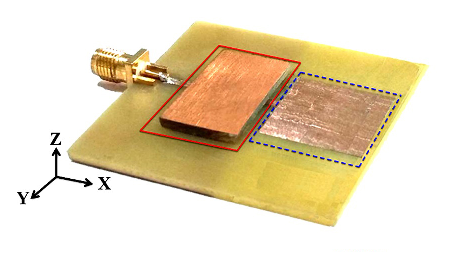
\includegraphics[width=0.4\linewidth]{Fig-aeue_2a.eps}}~~~~
\subfigure[]{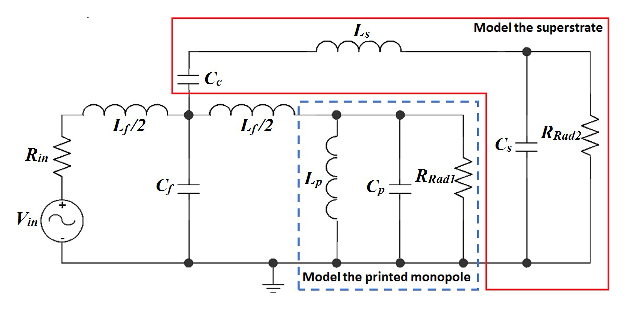
\includegraphics[width=0.6\linewidth]{Fig-aeue_2b.eps}}
\caption{(a) The fabricated antenna and (b) the equivalent circuit model of the antenna along with demarcations showing respective LCR sections for the printed monopole and the superstrate.}\label{FabEqckt}
\end{figure}

The values of the inductance and capacitance for a microstrip line are given by Equations \ref{eq_ind} and \ref{eq_cap} respectively \cite{multi_conductor_analysis_book}.

\begin{equation}\label{eq_ind}
L=
    \begin{cases}
    \frac{60l}{v_0}\ln\left[\frac{8h}{w}+\frac{w}{4h}\right]~~~~~~&\text{for}~\frac{w}{h}\leq1 \\
    \frac{120\pi l}{v_0}\left[\frac{1}{\frac{w}{h}+1.393+0.667\ln \left(\frac{w}{h}+1.444\right)}\right]~~~~~~&\text{for}~\frac{w}{h}>1
    \end{cases}
\end{equation}
\begin{equation}\label{eq_cap}
C=
\begin{cases}
    \frac{\epsilon_r l}{60v_0\ln\left[\frac{8h}{w}+\frac{w}{4h}\right]}~~~~~&\text{for}~\frac{w}{h}\leq1 \\
    \frac{\epsilon_r l\left[\frac{w}{h}+1.393+0.667 \ln\left(\frac{w}{h}+1.444\right)\right]}{120\pi v_0}~~~~~&\text{for}~\frac{w}{h}>1
\end{cases}
\end{equation}

Here, $l$ is the length of the microstrip line, $w$ is the width of the microstrip line, $\epsilon_r$ is the relative permittivity of the substrate material, $h$ is the height of the substrate and $v_0$ is the velocity of electromagnetic waves in free space. The values of $Ls$, $C_s$, $L_f$ and $C_f$ may be obtained from these equations.

For the printed monopole antenna, the values of $L_p$ and $C_p$ may be considered such that the resonant frequency of the antenna is equal to the resonant frequency of the LC tank circuit given by Equation \ref{eq_LC}.

\begin{equation}\label{eq_LC}
f_r = \frac{1}{2\pi \sqrt{L_p C_p}}
\end{equation}

Here, the resonant frequency of the printed monopole antenna is 2.4 GHz.

\section{Modeling and Analysis of the Proposed Antenna}\label{c4sec:analysis}
The mathematical expressions for estimating the values of the inductance and a capacitance of an equivalent circuit model are derived under many simplifying assumption \cite{handbook}. The accuracy of such empirical relationships is not high for practical antennas. In order to overcome these limitations, computational techniques are used. In the following sections, the parameters of the equivalent circuit model are estimated with Vector Fitting technique and the Genetic Algorithm.

\subsection{Analysis of the Equivalent Circuit Model with Vector Fitting Technique}
One of the techniques used for numerically estimating the equivalent circuit parameters of a printed antenna is vector fitting \cite{vectorfitting1, vectorfitting2, vectorfitting3}. Vector fitting technique models the frequency response of a system through rational function approximation. The rational function has a fixed number of poles and a residue part. This method was first proposed in \cite{vfit3_1}. An improved version of this technique is reported in \cite{vfit3_2} that uses relaxed non-triviality constraint for achieving faster convergence and higher accuracy. The present work uses the algorithm proposed in \cite{vfit3_3} where the differential equations are approximated as matrices for convenience of numerical implementation.

The Thevenin Equivalent load impedance of the equivalent circuit model can be expressed as Equation \ref{eq_Zin}.
{\small
\begin{equation}\label{eq_Zin}
Z_{L} = sL_f/2 + \left[\left(\frac{1}{sC_f}+sL_s+\left(\frac{1}{C_s} || R_{Rad2}\right)\right) || \left(\frac{1}{C_f}\right) || \left(sL_f/2 + \left(sL_p || \frac{1}{sC_p} || R_{Rad1}\right)\right)\right]
\end{equation}}
The return loss (S11) parameter can be calculated from the obtained value of $Z_{\text{in}}$ using Equation \ref{eq_Zin_s11}.

\begin{equation}\label{eq_Zin_s11}
S11\text{(dB)}=20 \log_{10}{\left(\left|\frac{Z_L - R_{\text{in}}}{Z_L + R_{\text{in}}}\right|\right)}
\end{equation}
Here, $R_{\text{in}}$ is the input impedance of the source. The typical value of $R_{\text{in}}$ is $50~\Omega$.

It can be shown that Equation \ref{eq_Zin} has seven poles. The vector fitting method is formulated to model a seven-pole system that can mimic the complex $Z_{\text{in}}$ parameter of the antenna obtained from simulation results over the entire observed band. The complex $Z_{\text{in}}$ plot is then converted to $S11$ parameter plot using Equation \ref{eq_Zin_s11} for the convenience of comparison and analysis. The seven poles obtained from this approach are enlisted in Table \ref{table_poles}.

\begin{table}
\centering
\caption{The poles of the equivalent circuit obtained from vector fitting}\label{table_poles}
\begin{tabular}{|c|c|c|c|}
  \hline
  Serial No & Real Part ($\sigma$) & Imaginary Part ($\omega$) & Equivalent Frequency (GHz) \\ \hline
 1 & -0.888 & 0.000 & 0.00 \\ \hline
 2 & -0.162 & 2.362 & 1.88 \\ \hline
 3 & -0.162 & -2.362 & -1.88 \\ \hline
 4 & -0.968 & 3.736 & 2.97 \\ \hline
 5 & -0.968 & -3.736 & -2.97 \\ \hline
 6 & -0.170 & 5.762 & 4.59 \\ \hline
 7 & -0.170 & -5.762 & -4.59 \\ \hline
\end{tabular}
\end{table}

It is observed from Table \ref{table_poles} that there is one pole at DC (frequency = 0.00 GHz) and three poles each at positive and negative frequencies. If we consider only the positive frequencies, the three poles are at 1.88 GHz, 2.97 GHz and 4.59 GHz.

\subsection{Estimation of the Equivalent Circuit Parameters Using Genetic Algorithm}
For simple circuits, it is possible to calculate the values of the lumped elements from the poles. For complex circuits, such computation is difficult and prone to errors. In recent years, soft-computational optimization algorithms such as genetic algorithm (GA), particle swarm optimization (PSO) etc. are widely used for modeling and optimization of printed antennas \cite{antSoftAppReview}. Here, genetic algorithm is used for estimating the equivalent circuit parameters of the antenna. The objective function in this case is defined in such a way that the resonant frequencies of the equivalent circuit remains nearest to the resonant frequencies of the antenna as obtained from full wave electromagnetic simulation. The parameters of the equivalent circuit model obtained from the genetic algorithm are shown in Table \ref{table_eqckt}.

\begin{table}
\centering
\caption{Values of the circuit parameters obtained from genetic algorithm}\label{table_eqckt}
\begin{tabular}{|l|c|}
\hline
Parameter & Value \\ \hline
Feed Inductance, $L_f$ & $1.00 \times 10^{-10}$ H \\ \hline
Feed Capacitance, $C_f$ & $4.133 \times 10^{-16}$ F \\ \hline
Printed Monopole Inductance, $L_p$ & $3.37 \times 10^{-9}$ H \\ \hline
Printed Monopole Capacitance, $C_p$ & $1.79 \times 10^{-12}$ F \\ \hline
Coupling Capacitance, $C_c$ & $1.41 \times 10^{-12}$ F \\ \hline
Superstrate Inductance, $L_s$ & $1.18 \times 10^{-9}$ H \\ \hline
Superstrate Capacitance, $C_s$ & $6.14 \times 10^{-13}$ F \\ \hline
\end{tabular}
\end{table}

\begin{figure}
\centering
\includegraphics[width=0.7\linewidth]{Fig-aeue_3.eps}
\caption{Comparison of the return loss (S11) parameter obtained from the equivalent circuit models using vector-fitting method and genetic algorithm with the return loss obtained from the full-wave simulation of the antenna.}\label{fig_vc_ga}
\end{figure}

Fig. \ref{fig_vc_ga} shows a comparison of the two equivalent circuit models in terms of the S11 parameter obtained. The S11 parameter plot of the equivalent circuit model in each case is compared with the S11 parameter plot obtained from full-wave simulation. It is observed that the vector fitting method provides a better estimation of the S11 parameter plot as compared to the genetic algorithm based approach.

\subsection{Current Analysis of the Equivalent Circuit Model of the Antenna}
The proposed equivalent circuit is simulated with a 1 Volt input source. The two load resistances $R_{Rad1}$ and $R_{Rad2}$ in the equivalent circuit model correspond to the radiation resistances of the printed monopole and the superstrate respectively. Thus, the current through $R_{Rad1}$ is an indicator of the power radiated from the printed monopole antenna and the current through $R_{Rad2}$ is an indicator of the power radiated from the superstrate. Fig. \ref{fig-ckt-current} (a) shows the current through $R_{Rad1}$ and $R_{Rad2}$ as obtained from the circuit simulation.

\begin{figure}
\centering
\subfigure[]{\includegraphics[width=0.6\linewidth]{Fig-aeue_4a.eps}}\\
\subfigure[]{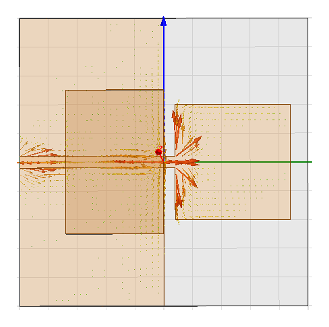
\includegraphics[width=0.3\linewidth]{Fig-aeue_4b.eps}}~~~
\subfigure[]{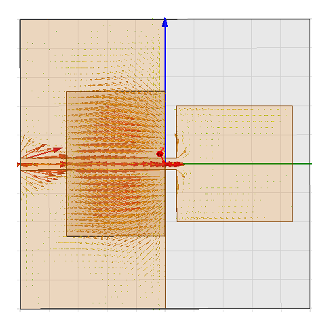
\includegraphics[width=0.3\linewidth]{Fig-aeue_4c.eps}}
\caption{(a) Current through $R_{Rad1}$ and $R_{Rad2}$ corresponding to the printed monopole antenna and the superstrate respectively. (b) Vector current density of the antenna at 2.4 GHz. (c) Vector current density of the antenna at 4.1 GHz.}\label{fig-ckt-current}
\end{figure}

It is observed that at 2.4 GHz, the current through $R_{Rad1}$, corresponding to the printed monopole antenna is high. The current through $R_{Rad2}$, corresponding to the superstrate is high near 4.5 GHz. However, at the resonant frequency of each section of the circuit, the current through the other part of the circuit also shows a local maximum point.

Here, the values of the circuit parameters obtained from the genetic algorithm are used for this analysis. The input resistance $R_{\text{in}}$ is fixed at 50 $\Omega$. This is the typical input impedance of an SMA connector, used for exciting a printed antenna. Both of the radiation resistances, $R_{Rad1}$ and $R_{Rad2}$ are fixed at 377 $\Omega$, which is the characteristic impedance of free space. Only the absolute value of the magnitude of the current is plotted.

The current density of the antenna obtained from full-wave simulation at 2.4 GHz and 4.1 GHz are shown in Figure \ref{fig-ckt-current} (b) and (c) respectively. It is observed that the current density is higher at the printed monopole antenna at 2.4 GHz and the current density is higher at the superstrate at 4.1 GHz. Thus, the equivalent circuit model perfectly explains the behavior of the antenna.

\section{Experimental Results and Discussions}\label{c4sec:expt_results}
This section covers the details of the experiments performed for determining the physical dimensions of the antenna and for evaluating its performance. These experiments include a parametric study of the antenna dimensions and evaluation of its resonant frequencies, gains, and radiation patterns through simulation and measurement.

\subsection{A Parametric Study of the Antenna Dimensions}
The physical dimensions of the antenna shown in Table \ref{table-dims} are tuned to study the influence of each dimension on the overall behavior of the antenna. Fig. \ref{fig-vars} shows the variation of the two resonant frequencies of the antenna with the length of the patch, $l_P$, the length of the superstrate, $l_S$, and the longitudinal spacing, $s$ between the superstrate and the patch. In each of the plots in Fig. \ref{fig-vars}, the other dimensions of the antenna are kept fixed as in Table \ref{table-dims}.

\begin{figure}[h]
\centering
\includegraphics[width=0.8\linewidth]{Fig-aeue_5.eps}
\caption{Variation of resonant frequency of the antenna with the (a) length of the patch, $L_P$, (b) length of the superstrate, $L_s$ (c) Spacing, $S$ between the superstrate and the patch.}\label{fig-vars}
\end{figure}

Fig. \ref{fig-vars} (a) shows that as the length of the patch increases, both the resonant frequencies of the antenna falls almost linearly. The length of the superstrate has a more impact on the second resonant frequency as a decreasing trend is observed from Fig. \ref{fig-vars} (b) for $l_S~>~17mm$. This observation clearly indicats the effect of the superstrate on the second resonant frequency of the antenna. The variation of the resonant frequencies of the antenna with $s$ is shown in Fig. \ref{fig-vars} (c). The desired resonant frequency and radiation pattern of the antenna are obtained for $s~=~2mm$.

\subsection{Return Loss Measurement}
\begin{figure}
\centering
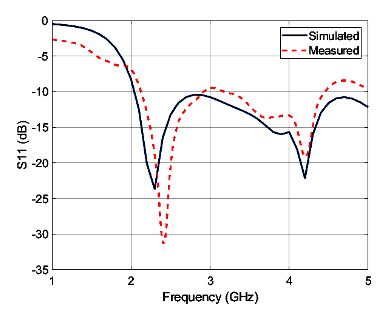
\includegraphics[width=0.5\linewidth]{Fig-aeue_6.eps}
\caption{The simulated and measured return loss (S11) parameter plot of the proposed antenna}\label{fig-s11}
\end{figure}

The simulated and the measured return loss (S11) parameter plot of the proposed antenna is shown in Fig. \ref{fig-s11}. The measurements are performed with a Rhode \& Schwarz ZNB-20 vector network analyzer (VNA). The antenna has two distinct wide operating bands. The first operating band covers the 2.4 GHz ISM band and the second resonant frequency covers the C-band of 5G wireless communication from 3.5 GHz to 4.2 GHz. The measurement result closely follows the simulation result with a minor deviation that may be attributed to an imperfection in the tolerance of fabrication.

\subsection{Radiation Pattern and Gain Measurement}
The co-polar and the cross-polar radiation patterns are measured for both the principal plane of the antenna at its peak resonant frequencies. The measurements are carried out with a standard horn antenna as the transmitter and the antenna under test on a turn table interfaced with the VNA. The measured radiation patterns are shown in Fig. \ref{fig-pat}. It is observed that the antenna provides an omnidirectional radiation pattern in the YZ-plane at 2.4 GHz and a directional radiation pattern in the YZ-plane at 4.2 GHz. The peak gains achieved at 2.4 GHz and 4.2 GHz are 3.1 dBi and 5.1 dBi respectively. All planes used for describing the radiation patterns are in accordance with the orientation of the antenna as shown in Fig. \ref{FabEqckt} (a).

\begin{figure}[h]
\centering
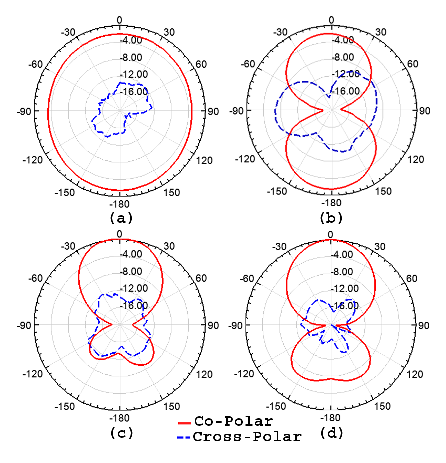
\includegraphics[width=0.5\linewidth]{Fig-aeue_7.eps}
\caption{Radiation pattern of the antenna in the (a) YZ Plane at 2.4 GHz (b) XZ Plane at 2.4 GHz, (c) YZ Plane at 4.2 GHz, (d) XZ Plane at 4.2 GHz}\label{fig-pat}
\end{figure}

\section{Discussions and Conclusion}\label{c4sec:concl}
From the analysis and the experimental results it is observed that the proposed antenna has two distinct far-field radiation patterns at its two resonant frequencies. An equivalent circuit model of the antenna is also proposed. The behavior of the antenna is explained with the equivalent circuit model. The parameters of the equivalent circuit model are obtained using vector-fitting technique and genetic algorithm. The accuracy of the equivalent circuit model is validated through comparison of its output current with the simulation results of the antenna.

The proposed antenna has an omnidirectional radiation pattern at the 2.4 GHz ISM band. At the C-band, the primary radiating element is the superstrate and the antenna has a directional radiation pattern with a higher gain due to the presence of the ground plane. At this band, the antenna is more suitable for directional communication. The antenna finds its possible applications in an IoT or WiFi network with a 5G backbone. 